\documentclass[]{article}
\usepackage{upquote}
\usepackage{listings}
\usepackage{color}
\usepackage[margin=1cm]{geometry}
 \usepackage{graphicx}
%\usepackage{wrapfig}
\begin{document}

\title{NewzTrader: Autonomous Trading Agent Implementation Using Natural Language Processing Of News Headlines}
\author{William Lyon}
\date{\today}
\maketitle

\abstract{Natural Language Processing techniques are used to examine financial news headlines and generate predictions of stock price movements.  News headlines from the Wall Street Journal from January 1, 2009 to November 1, 2012 are collected and paired with daily S\&P 500 index returns.  This information is used to train a Naive Bayes classifier and generate BUY/SELL trading signals.  This trading strategy is then backtested using Wall Street Journal news headlines as a predictor for movement in the price of the S\&P 500 index. }

\section{Introduction}
In finance, the Efficient Market Hypothesis states that all publicly available information is reflected in financial market prices.  As new information becomes available, prices adjust to take this new information into account.  
\subsection{Motivation}
This tool could be used as a component of an autonomous trading agent that will make BUY/SELL decisions for trading financial instruments.

Goals: 1) 
\subsection{Literature Review}

\section{Examining The Data}
Google Finance provides access to historical stock quotes as well as links to financial news stories pertaining to specific stocks. This data provides the basis for this paper.
\subsection{Historical Stock Market Quotes}
\subsection{News Headlines}
A total of 101,618 news headlines over 1416 days were collected with an average of 71 headlines per day.  After aligning with financial data:
UP: 14651
DOWN: 13718
NONE: 57405
TOTOAL: 85775

Prior probs:
UP: 0.1708
DOWN: 0.1599
NONE:  0.6693

\begin{figure}[h!]
%\begin{wrapfigure}{o}{8cm}
\centering
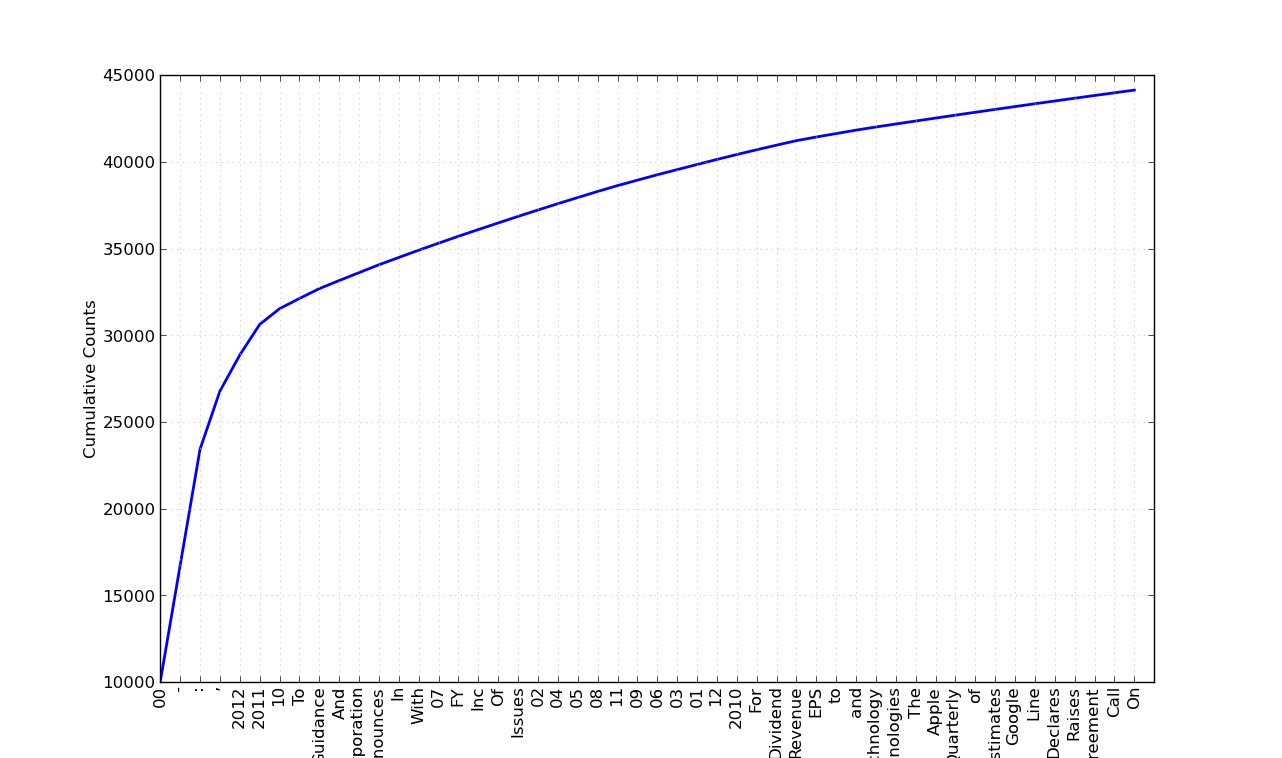
\includegraphics[scale=0.25]{cum_graph.png}
\caption{Cumulative frequency plot}
\end{figure}
%\end{wrapfigure}
%\end{figure}
%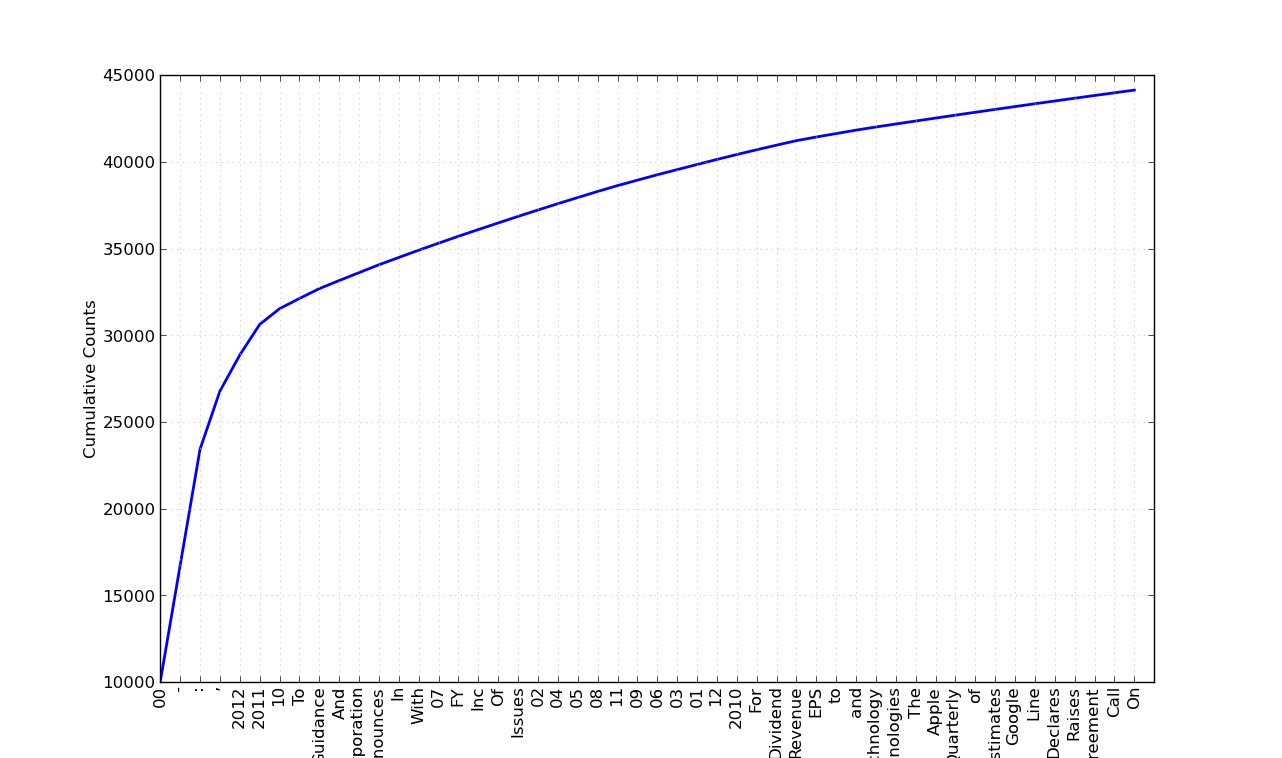
\includegraphics[width=60mm]{cum_graph.png}
%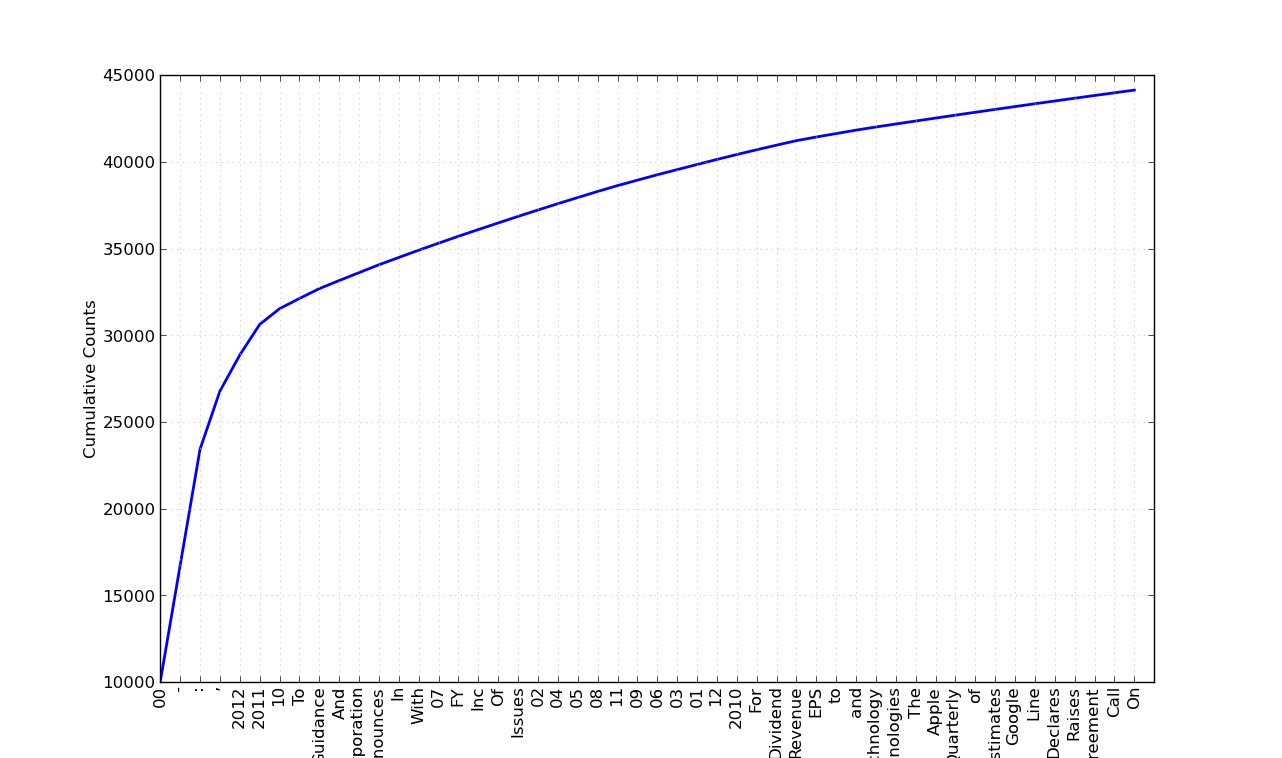
\includegraphics[height=60mm]{cum_graph.jpg}
%\includegraphics[scale=0.75]{myfig.pdf}
%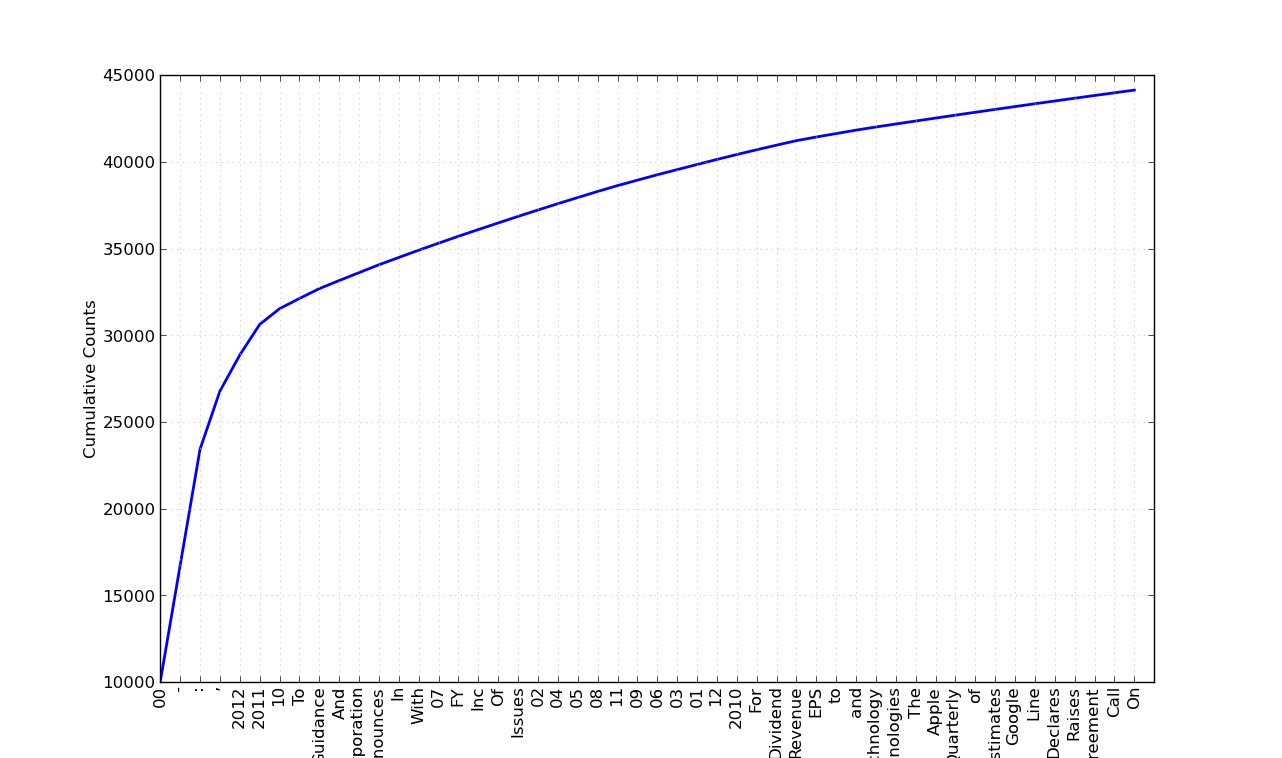
\includegraphics[angle=45,width=52mm]{cum_graph.png}
\section{Classification Methodology}
These tuples of [return, listOfDailyNews] are used as the training data for a Naive Bayes classifier. 
\subsection{Classes}

\subsection{Naive Bayes}
\subsection{Maximum Entropy}

\section{Implementation}

\subsection{Dependencies}
\subsection{Data Collection \& Munging}
\subsection{Feature Extraction}
\subsubsection{Bag of words}
\subsubsection{Filtering stopwords}
\subsubsection{Include significant bigrams}


\subsection{Naive Bayes Classifier}
\subsection{Maximum Entropy Classifier}
\subsection{Backtesting}
\section{Evaluation}
\subsection{Accuracy}

\subsection{Most informative features}

\subsection{Precision}

\subsection{Recall}

\section{Trading Model}
\subsection{Trading Signals}
\subsection{Backtesting}
This is the backtestinfg. Where is the rest of the backtesting?

\section{Conclusions}
These are my conclusions. Where are the conclusions/

\subsection{Further research}

\section{References}

\onecolumn
\section{Source Code Listings}

\lstset{frame=shadowbox, numbers=left, float, caption=newsCredScraper.py: scrapes WSJ news headlines, language=Python, breaklines=True, columns=fullflexible, rulesepcolor=\color{blue}}
\lstinputlisting{src/newsCredScraper.py}

\lstset{frame=shadowbox, numbers=left, float, caption=dataGetter.py: downloads historical S\&P 500 index price data and joins with WSJ news  headlines / identifies news headline classifications and saves in format for corpus reader, language=Python, breaklines=True, columns=fullflexible, rulesepcolor=\color{blue}}
\lstinputlisting{src/dataGetter.py}

\lstset{frame=shadowbox, numbers=left, float, caption=nbTrainer.py: loads news corpus / trains Naive Bayes classifier, language=Python, breaklines=True, columns=fullflexible, rulesepcolor=\color{blue}}
\lstinputlisting{src/nbTrainer.py}

\lstset{frame=shadowbox, numbers=left, float, caption=backTest.py: simulates trading using trading signals generated from WSJ news headlines using Naive Bayes classifier, language=Python, breaklines=True, columns=fullflexible, rulesepcolor=\color{blue}}
\lstinputlisting{src/backTest.py}

\lstset{frame=shadowbox, numbers=left, float, caption=NewzTrader.py, language=Python, breaklines=True, columns=fullflexible, rulesepcolor=\color{blue}}
\lstinputlisting{src/NewzTrader.py}

\end{document}